%
%
%% Enter Figures and Tables here:
%
% DO NOT USE \psfrag or \subfigure commands.
%
% Figure captions go below the figure.
% Table titles go above tables; all other caption information
%  should be placed in footnotes below the table.
%
%----------------
% BEGIN FIGURES
%----------------

%%%%%%%%%%%%%%%%%%%%%%%%%%%
%%%%%%% CLIMATE %%%%%%%%%%%
%%%%%%%%%%%%%%%%%%%%%%%%%%%

\clearpage
\begin{figure}[t]
  \begin{center}
    \includegraphics[width=1\textwidth,angle=0.]{./figs/f_CAM_CESM_NMSE_DJF_JJA.pdf}
 \end{center}
  \caption {Climatology of contributions to the Normalized Mean Square Error (NMSE) over the northern hemisphere (30$^\circ$ N-90$^\circ$ N) for CAM releases between CAM3 and CAM6 during (a) DJF (December/January/February) and (b) JJA (June/July/August). Individual contributions are from the unconditional bias (hatched), conditional bias (solid) and phase error (unfilled). The narrow unfilled bar for each model is the scaled variance ratio (SVR), which is larger than the NMSE if the modeled variance is inflated compared to observed. Model biases are referenced to the ECMWF (ERA15) reanalysis. Contemporary analysis JRA25 \citep{ONOGI2007}, NCEP \citep{Kanamitsu2002}, ERA40 \citep{Uppala2005} and ERA-interim \citep{Dee2011} differences compared to ECMWF \citep{Gibson1997} are also shown.} 
\label{f_CAM_CESM_NMSE_DJF_JJA}
\end{figure} 

%%
\clearpage
\begin{figure}[t]
  \begin{center}
    \includegraphics[width=1.\textwidth,angle=0.]{./figs/f_TAYLOR_CAM_CESM.png}
  \end{center}
  \caption{Taylor diagrams \citep{Taylor2001} for AMIP (CAM4/CAM5/CAM6) and fully coupled (CCSM4/CESM1/CESM) annual climatology simulation performance.}
\label{f_TAYLOR_CAM_CESM}
\end{figure}

%%
\clearpage
\begin{figure}[t]
  \begin{center}
    \includegraphics[width=1.\textwidth,angle=0.]{./figs/f_PRECT_2D_CAM456.pdf}
  \end{center}
  \caption{Climatology of annual precipitation (mm/day) for (a) Observations (GPCP, 1979-2007), and biases for (b) CAM6, (c) CAM5, and (d) CAM4 AMIP simulations for the period 1979-2005. Hatched areas are where wet biases exceed 100\% of observed and vertical line regions are where dry biases are less than 25\% of observed.}
\label{f_PRECT_2D_CAM456}
\end{figure}
%%
\clearpage
\begin{figure}[t]
%  \begin{center}
    \includegraphics[width=1.\textwidth,angle=0.]{./figs/f_PRECT_1D_DJF_CAM456.pdf}
%  \end{center}
  \caption{Climatology of DJF precipitation (mm/day) for (a) Observations (GPCP, 1979-2007 and CAM AMIP simulations (1979-2005) and (b) the AMIP (dash) and equivalent} 
\label{f_PRECT_1D_DJF_CAM456}
\end{figure} 

%%
\clearpage
\begin{figure}[t]
  \begin{center}
    \includegraphics[width=1.\textwidth,angle=0.]{./figs/f_PRECT_1D_JJA_CAM456.pdf}
  \end{center}
  \caption{Climatology of JJA precipitation (mm/day) for (a) Observations (GPCP, 1979-2007), and its biases for (a) CAM4 (b) CAM5  through CAM6 AMIP simulations for the period 1979-2005} 
\label{f_PRECT_1D_JJA_CAM456}
\end{figure} 


%%
\clearpage
\begin{figure}[t]
  \begin{center}
    \includegraphics[width=0.55\textwidth,angle=90.]{./figs/f_PSICHI_2D_DJF_CAM456_diff.pdf}
  \end{center}
  \caption{Climatology of annual precipitation (mm/day) for (a) Observations (GPCP, 19XX-20XX), and its biases for (a) CAM4 (b) CAM5  through CAM6 AMIP simulations for the period 1979-2005. Hatched areas are where wet biases exceed 100\% of observed and vertical line regions are where dry biases are greater than 25\% of observed.}
\label{f_PSICHI_2D_DJF_CAM456_diff}
\end{figure}

%%
\clearpage
\begin{figure}[t]
  \begin{center}
    \includegraphics[width=1.\textwidth,angle=0.]{./figs/f_SWCF_2D_CAM456_ANN.pdf}
  \end{center}
  \caption{Climatology of annual  (mm/day) for (a) Observations (GPCP, 19XX-20XX), and its biases for (a) CAM4 (b) CAM5  through CAM6 AMIP simulations for the period 1979-2005. Hatched areas are where wet biases exceed 100\% of observed and vertical line regions are where dry biases are greater than 25\% of observed.}
\label{f_SWCF_2D_CAM456}
\end{figure}




%%
\clearpage
\begin{figure}[t]
%  \begin{center}
    \includegraphics[width=1.\textwidth,angle=0.]{./figs/f_LWCF_1D_ANN_CAM456.pdf}
%  \end{center}
  \caption{Climatology of annual precipitation (mm/day) for (a) Observations (GPCP, 19XX-20XX), and its biases for (a) CAM4 (b) CAM5  through CAM6 AMIP simulations for the period 1979-2005} 
\label{f_LWCF_1D_ANN_CAM456}
\end{figure} 

%%
\clearpage
\begin{figure}[t]
  \begin{center}
    \includegraphics[width=1.1\textwidth,angle=0.]{./figs/f_MMC_2D_ANN_CAM456.pdf}
  \end{center}
  \caption{Climatology of annual mean meridional circulation (units) for (a) Observations (ERA-interim 19XX-20XX) and biases for (b) CAM6, (c) CAM5 and (d) CAM4.} 
\label{f_MMC_2D_ANN_CAM456}
\end{figure} 


%%
\clearpage
\begin{figure}[t]
%  \begin{center}
    \includegraphics[width=1.\textwidth,angle=0.]{./figs/f_T_2D_ANN_CAM456.pdf}
%  \end{center}
  \caption{Climatology of annual mean temperature (K) for (a) Observations (GPCP, 19XX-20XX), and its biases for (a) CAM4 (b) CAM5  through CAM6 AMIP simulations for the period 1979-2005} 
\label{f_T_2D_ANN_CAM456}
\end{figure} 




%%
\clearpage
\begin{figure}[t]
  \begin{center}
    \includegraphics[width=1.\textwidth,angle=0.]{./figs/f_MERRA_Q_latp_diff_ANN.pdf}
  \end{center}
  \caption{Climatology of annual precipitation (mm/day) for (a) Observations (GPCP, 19XX-20XX), and its biases for (a) CAM4 (b) CAM5  through CAM6 AMIP simulations for the period 1979-2005} 
\label{MERRA_Q_latp_diff_ANN}
\end{figure} 

%%
\clearpage
\begin{figure}[t]
  \begin{center}
    \includegraphics[width=1.\textwidth,angle=0.]{./figs/f_U_2D_ANN_CAM456.pdf}
  \end{center}
  \caption{Climatology of annual mean zonal wind) Observations (GPCP, 19XX-2007), and its biases for (a) CAM4 (b) CAM5  through CAM6 AMIP simulations for the period 1979-2005} 
\label{f_U_2D_ANN_CAM456}
\end{figure} 


%%%%%%%%%%%%%%%%%%%%%%%%%%%
%%%%%%% TENDENCIES %%%%%%%%
%%%%%%%%%%%%%%%%%%%%%%%%%%%


%%
\clearpage
\begin{figure}[t]
  \begin{center}
    \includegraphics[width=0.9\textwidth,angle=0.]{./figs/f_dqdt_pbl_2d_cam6_ann.pdf}
  \end{center}
  \caption{Annual climatology of CAM6 tendencies of humidity from the primary physical process parameterizations vertically averaged between the surface and 800 hPa.} 
\label{f_dqdt_pbl_2d_cam6_ann}
\end{figure} 

%%
\clearpage
\begin{figure}[t]
  \begin{center}
    \includegraphics[width=0.6\textwidth,angle=90.]{./figs/f_dqdt_pbl_2d_cam5_ann.pdf}
  \end{center}
  \caption{Annual climatology of CAM5 tendencies of humidity from the primary physical process parameterizations vertically averaged between the surface and 800 hPa.} 
\label{f_dqdt_pbl_2d_cam5_ann}
\end{figure} 
%%
\clearpage
\begin{figure}[t]
  \begin{center}
    \includegraphics[width=0.55\textwidth,angle=90.]{./figs/f_prof_regions.pdf}
  \end{center}
  \caption{Location of state and tendency regions used for profile analysis of the CAM release simulations} 
\label{f_prof_regions}
\end{figure} 
%%
\clearpage
\begin{figure}[t]
  \begin{center}
    \includegraphics[width=0.25\textwidth,angle=90.]{./figs/f_vprof_nitcz_JJA.pdf}
  \end{center}
  \caption{Vertical profiles of JJA climatology for CAM4, CAM5, CAM6 and observations of (a) equivalent potential temperature (THE, K), relative humidity (RELHUM, \%), total cloud fraction (CLOUD, \%) and (grid box average cloud liquid (CLDLIQ, g/kg). Data is averaged over the "Northern ITCZ" region.} 
\label{f_vprof_nitcz_JJA}
\end{figure} 

%%
\clearpage
\begin{figure}[t]
  \begin{center}
    \includegraphics[width=0.25\textwidth,angle=90.]{./figs/f_vprof_wio_JJA.pdf}
  \end{center}
  \caption{Vertical profiles of JJA climatology for CAM4, CAM5, CAM6 and observations of (a) equivalent potential temperature (THE, K), relative humidity (RELHUM, \%), total cloud fraction (CLOUD, \%) and (grid box average cloud liquid (CLDLIQ, g/kg). Data is averaged over the "Western Indian Ocean" region.} 
\label{f_vprof_wio_JJA}
\end{figure} 

%%
\clearpage
\begin{figure}[t]
  \begin{center}
    \includegraphics[width=0.25\textwidth,angle=90.]{./figs/f_vprof_epac_JJA.pdf}
  \end{center}
  \caption{Vertical profiles of JJA climatology for CAM4, CAM5, CAM6 and observations of (a) equivalent potential temperature (THE, K), relative humidity (RELHUM, \%), total cloud fraction (CLOUD, \%) and (grid box average cloud liquid (CLDLIQ, g/kg). Data is averaged over the "East Pacific" region.} 
\label{f_vprof_epac_JJA}
\end{figure} 


%%
\clearpage
\begin{figure}[t]
  \begin{center}
    \includegraphics[width=0.25\textwidth,angle=90.]{./figs/f_vprof_socn_JJA.pdf}
  \end{center}
  \caption{Vertical profiles of JJA climatology for CAM4, CAM5, CAM6 and observations of (a) equivalent potential temperature (THE, K), relative humidity (RELHUM, \%), total cloud fraction (CLOUD, \%) and (grid box average cloud liquid (CLDLIQ, g/kg). Data is averaged over the "Southern Ocean" region.} 
\label{f_vprof_socn_JJA}
\end{figure} 


%%
\clearpage
\begin{figure}[t]
  \begin{center}
    \includegraphics[width=0.9\textwidth,angle=0.]{./figs/f_vtend_DQDT_CAM6.pdf}
  \end{center}
  \caption{Vertical profiles of CAM6 moist physics humidity tendencies (g/kg/day) for JJA, 1979-2005 over the regions identified in Fig.\ref{f_prof_regions}.} 
\label{f_vtend_DQDT_CAM6}
\end{figure} 

%%
\clearpage
\begin{figure}[t]
  \begin{center}
    \includegraphics[width=0.9\textwidth,angle=0.]{./figs/f_vtend_DQDT_CAM5.pdf}
  \end{center}
  \caption{Vertical profiles of CAM5 moist physics humidity tendencies (g/kg/day) for JJA, 1979-2005 over the regions identified in Fig. \ref{f_prof_regions}.} 
\label{f_vtend_DQDT_CAM5}
\end{figure} 


%%%%%%%%%%%%%%%%%%%%%%%%%%%
%%%%%%% SENSITIVITIES %%%%%
%%%%%%%%%%%%%%%%%%%%%%%%%%%
%%%%% REGIONAL BIAS/RMSE %%%%%
%%
\clearpage
\begin{figure}[t]
  \begin{center}
    \includegraphics[width=0.5
    \textwidth,angle=90.]{./figs/f_scatt_tropics_PRECT_ocean.pdf}
  \end{center}
  \caption{Scatter plot of seasonal precipitation root mean squared error and bias (mm/day) over tropical land for a selection of baseline and revert experiments. Revert experiments are described in table \ref{t1}} 
\label{f_scatt_tropics_PRECT_ocean}
\end{figure} 

%%
\clearpage
\begin{figure}[t]
  \begin{center}
    \includegraphics[width=0.5\textwidth,angle=90.]{./figs/f_scatt_tropics_PRECT_land.pdf}
  \end{center}
  \caption{Scatter plot of seasonal precipitation root mean squared error and bias (mm/day) over tropical land for a selection of baseline and revert experiments. Revert experiments are described in table \ref{t1}} 
\label{f_scatt_tropics_PRECT_land}
\end{figure} 




%%%%% ZONAL AVERAGES %%%%%%
%%
\clearpage
\begin{figure}[t]
  \begin{center}
    \includegraphics[width=0.45\textwidth,angle=90.]{./figs/f_revert_PRECT_1D.pdf}
  \end{center}
  \caption{Zonal average precipitation (mm/day) for a number of parameter and parameterization revert experiments for (a) DJF and (b) JJA climatologies. Revert experiments are described in table \ref{t1}} 
\label{f_revert_PRECT_1D}
\end{figure} 

%%
\clearpage
\begin{figure}[t]
  \begin{center}
    \includegraphics[width=0.45\textwidth,angle=90.]{./figs/f_revert_LHFLX_1D.pdf}
  \end{center}
  \caption{Zonal average latent heat flux (Wm$^{-2}$) in CAM6 parameter and parameterization revert experiments for (a) DJF and (b) JJA climatologies (1979-2005). Revert experiments are described in table \ref{t1}} 
\label{f_revert_LHFLX_1D}
\end{figure} 

%% REGIONAL TENDENCIES %%
\clearpage
\begin{figure}[t]
  \begin{center}
    \includegraphics[width=1.1\textwidth,angle=0.]{./figs/f_revert_PRECT_2D.png}
  \end{center}
  \caption{Precipitation (mm/day) for DJF (left column) and JJA (right column) in (a) C6:CAM6 and anomalies from CAM6 in (b) rC5: Revert to CAM5 physics, (c) rUW: Revert to UW schemes, (d) rMG1: Revert to MG1 microphysics, (e) rC5pm: Revert primary tuning parameters back to CAM5 (f) rpfrac: Revert to FULL OVERLAP precipitation method, (g) rZMc: Revert to ZM convection capeten=5 setting}   
\label{f_revert_PRECT_2D}
\end{figure} 

&&
\clearpage
\begin{figure}[t]
  \begin{center}
    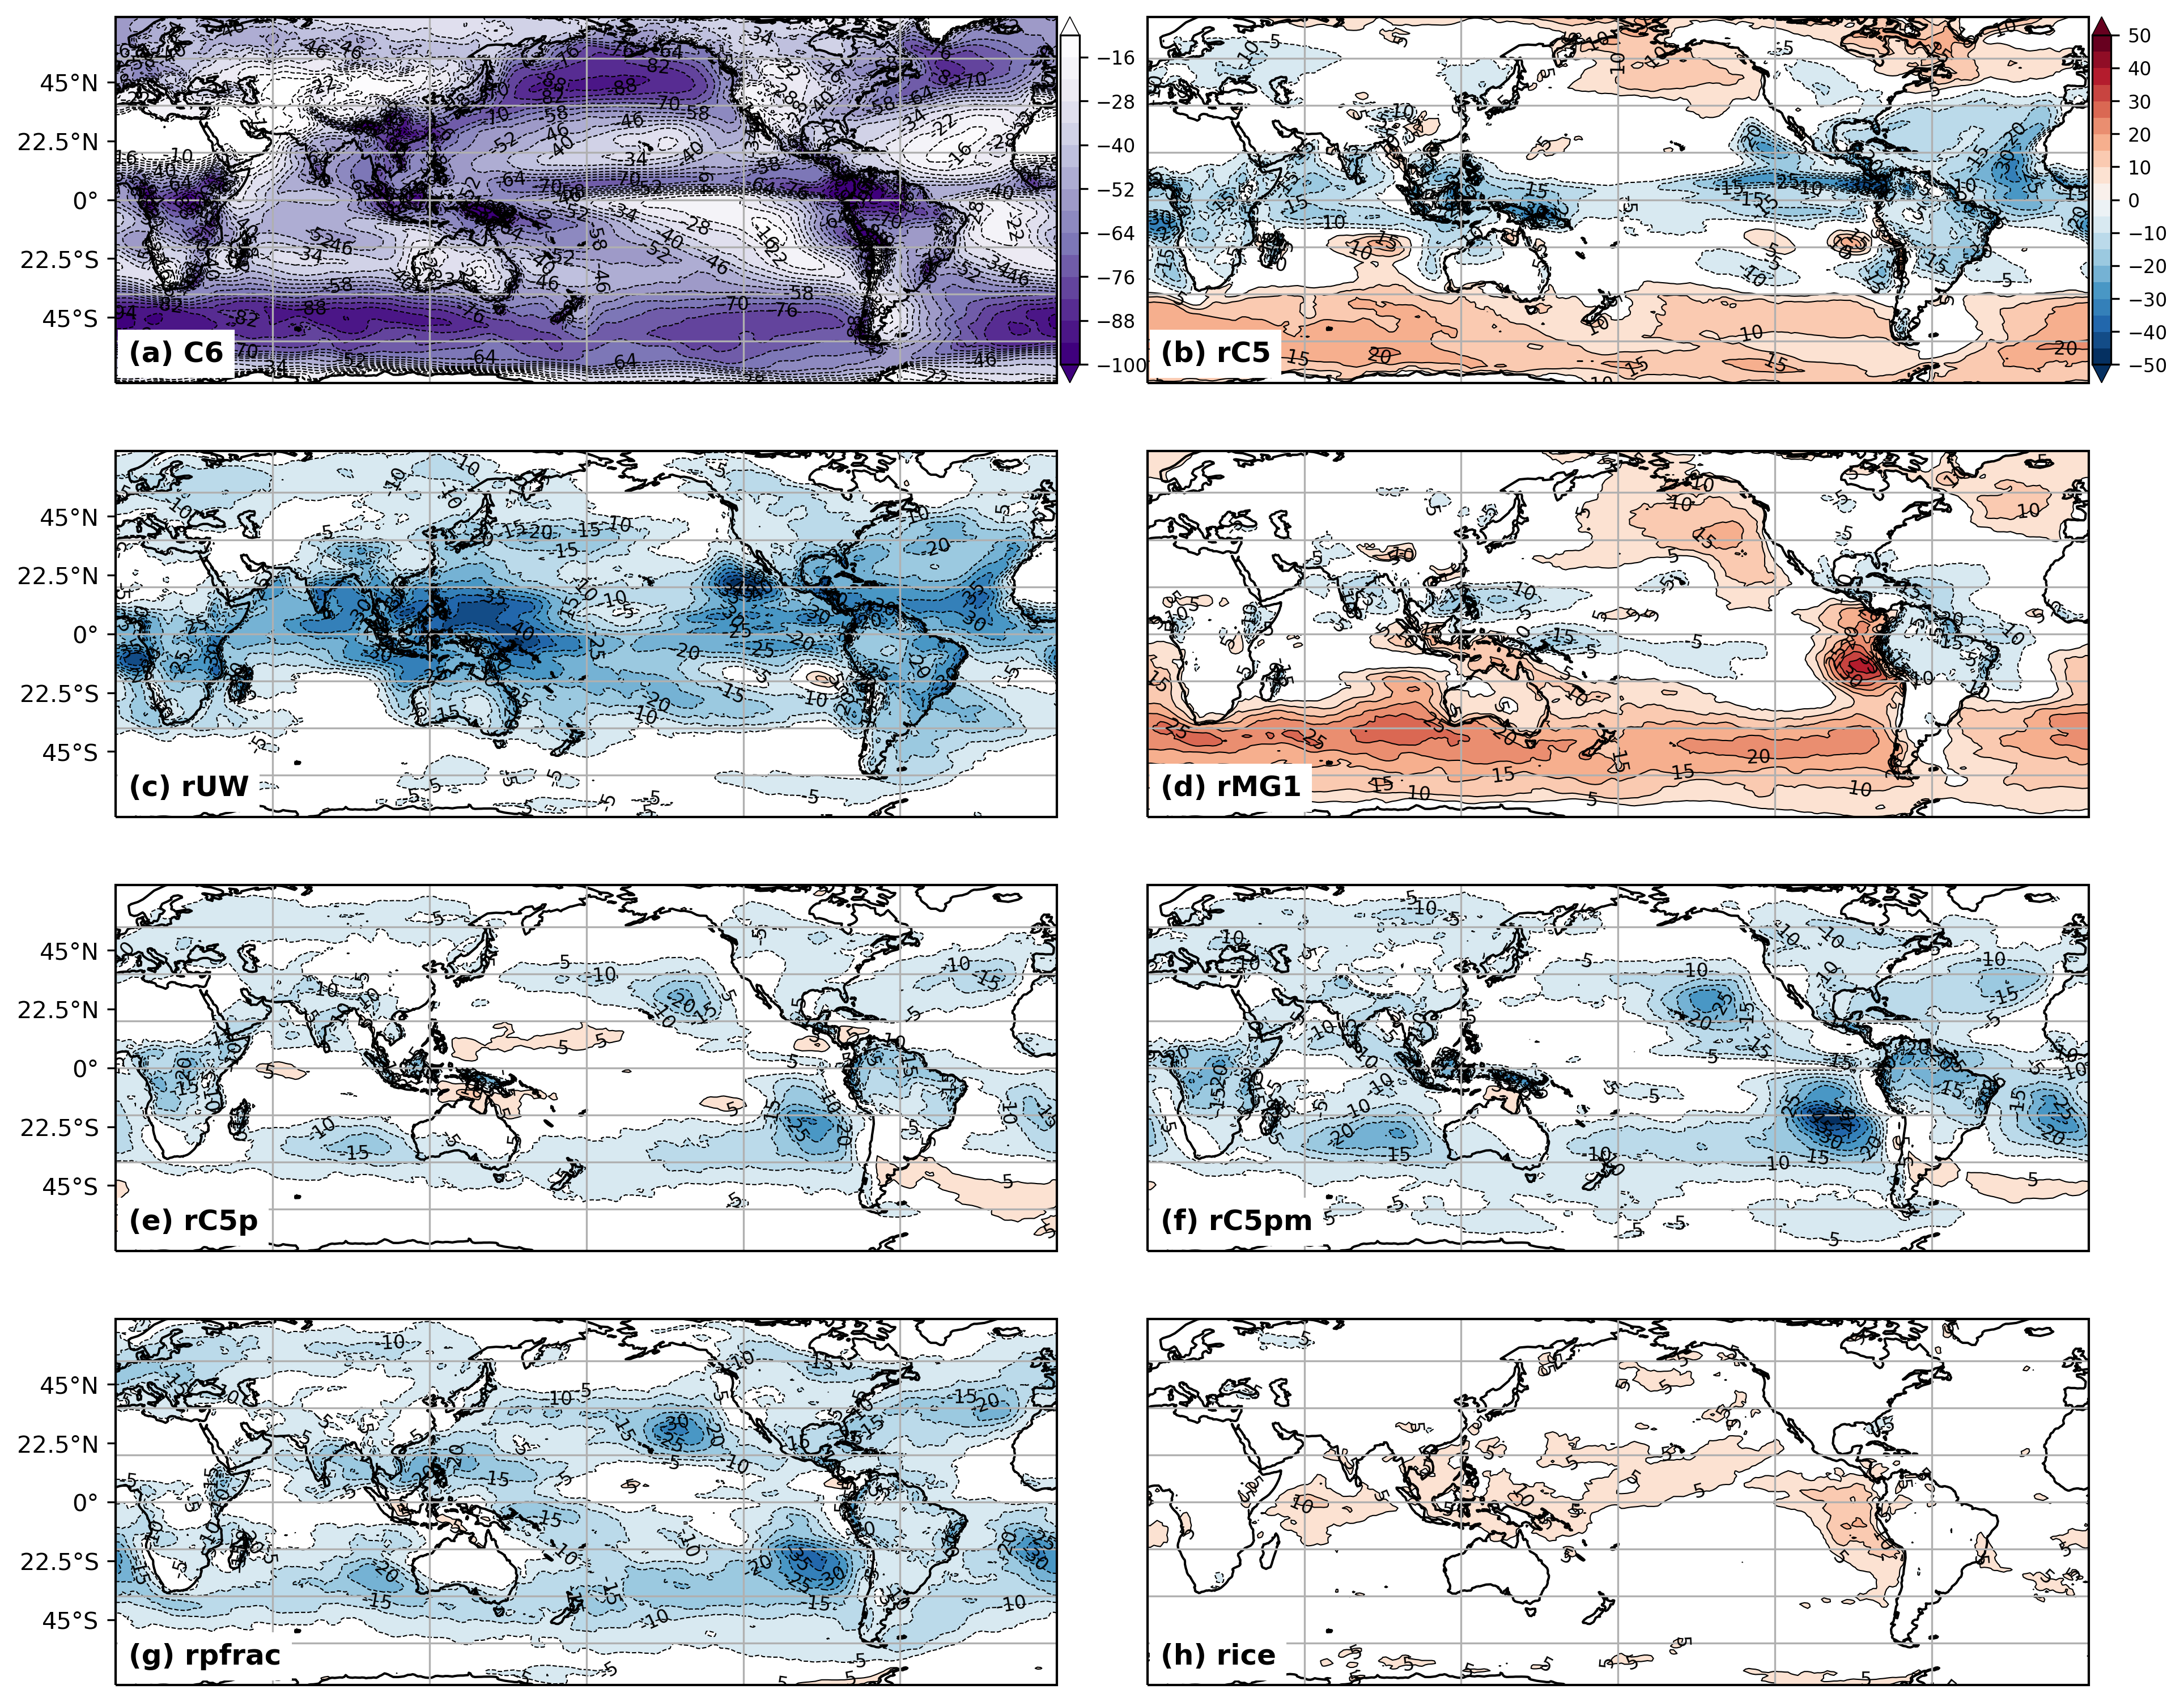
\includegraphics[width=1.1\textwidth,angle=0.]{./figs/f_revert_SWCF_ANN_2D.png}
  \end{center}
  \caption{Revert SWCF ANN} 
\label{f_revert_SWCF_ANN_2D}
\end{figure} 
&&
\clearpage
\begin{figure}[t]
  \begin{center}
    \includegraphics[width=1.1\textwidth,angle=0.]{./figs/f_revert_LWCF_ANN_2D.png}
  \end{center}
  \caption{Revert SWCF ANN} 
\label{f_revert_LWCF_ANN_2D}
\end{figure} 
&&
\clearpage
\begin{figure}[t]
  \begin{center}
    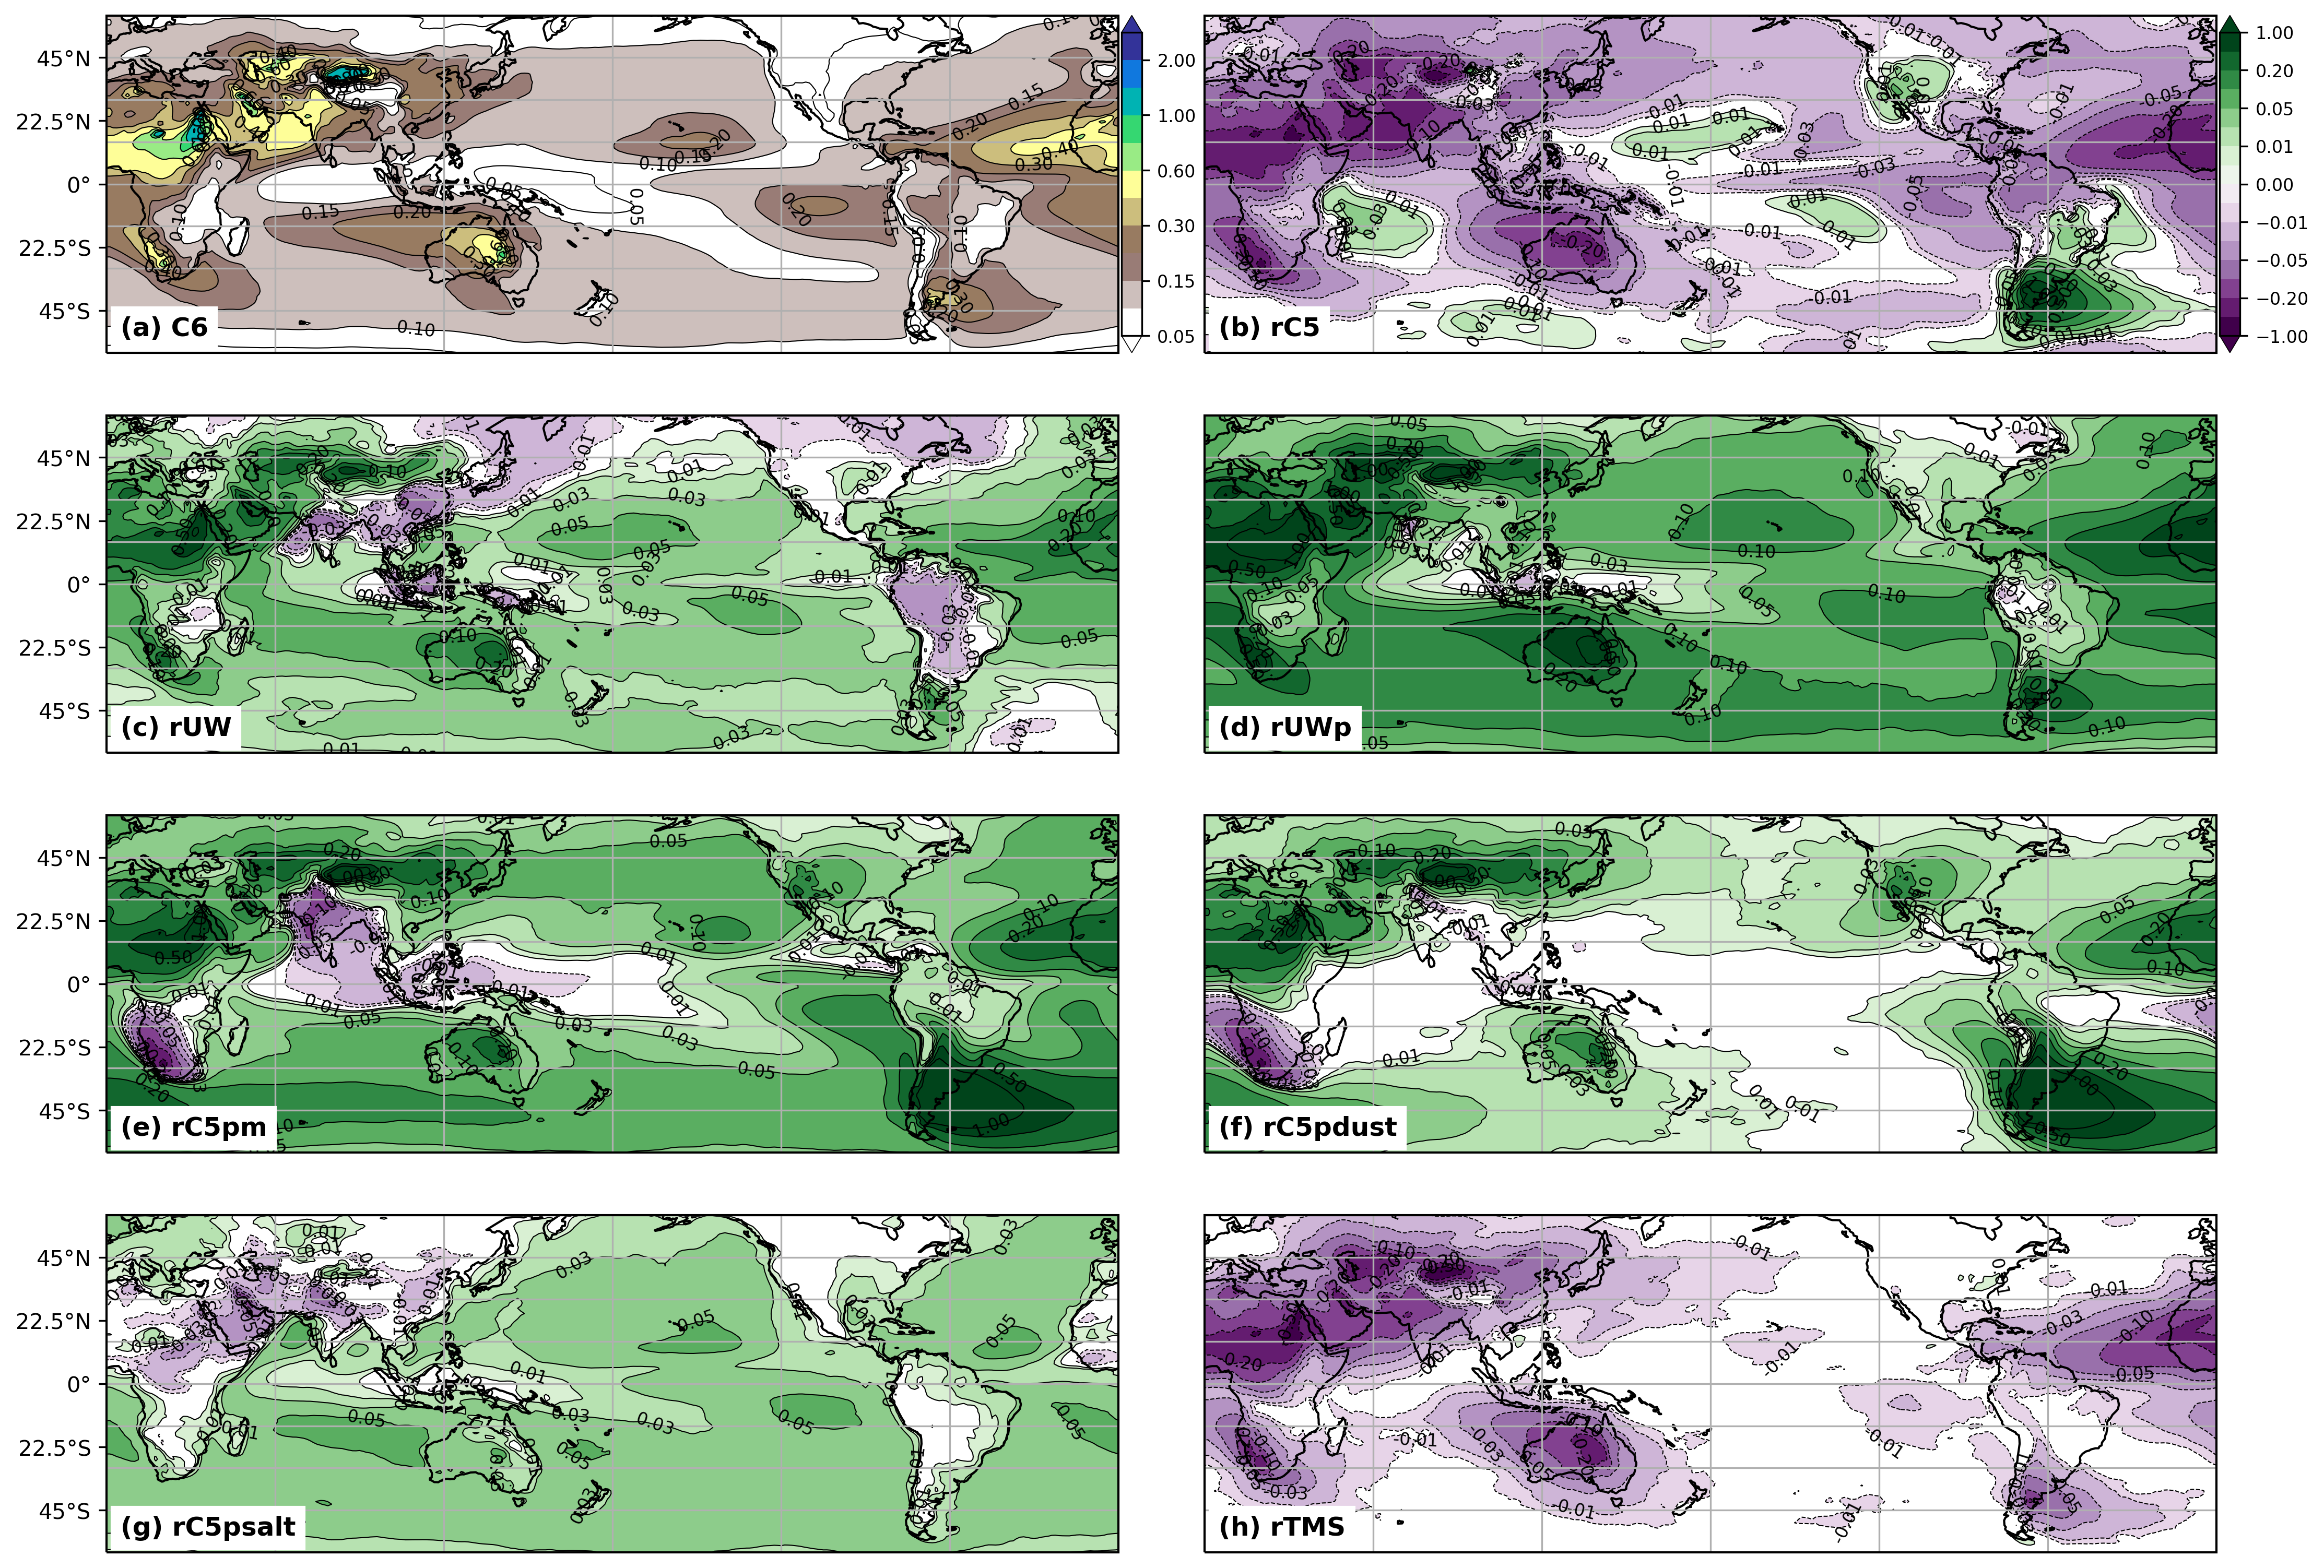
\includegraphics[width=1.1\textwidth,angle=0.]{./figs/f_revert_AODVIS_ANN_2D.png}
  \end{center}
  \caption{Revert SWCF ANN} 
\label{f_revert_AODVIS_ANN_2D}
\end{figure} 
\clearpage
&&
\begin{figure}[t]
  \begin{center}
    \includegraphics[width=1.1\textwidth,angle=0.]{./figs/f_revert_U_2D.png}
  \end{center}
  \caption{Annual mean zonally averaged zonal wind (m/s) for (a) C6:CAM6 and anomalies from CAM6 in (b) rC5: Revert to CAM5 physics, (c) rUW: Revert to UW schemes, (d) rMG1: Revert to MG1 microphysics, (e) rC5pm: Revert primary tuning parameters back to CAM5 (f) rpfrac: Revert to FULL OVERLAP precipitation method, (g) rZMc: Revert to ZM convection capeten=5 setting}   
\label{f_revert_U_2D}
\end{figure} 

&&


%%%%%%%%%%%%%

